\documentclass{article}
\usepackage[utf8]{inputenc}
\usepackage{latexsym}
\usepackage{url}
\usepackage{hyperref}
\usepackage{graphicx}
\usepackage[table]{xcolor}
\usepackage[T1]{fontenc} 
\usepackage{LobsterTwo}
\usepackage{amsmath} %for math operations
\usepackage{fancyhdr} %for page style
\usepackage{lastpage} %for no of page
\usepackage[a4paper, total={6in, 8in}]{geometry} %for margins
\usepackage{geometry}
\geometry{right=24mm,left=24mm,top=45mm,bottom=45mm} %for page size 
\usepackage{bookman}
\usepackage{wrapfig}
\usepackage{multirow}
\usepackage{tabularx}
\usepackage{amssymb}
\usepackage[ruled, linesnumbered]{algorithm2e}    
\usepackage{algorithm}
\hypersetup{
     colorlinks=true, % make the links colored
     linkcolor=red,   % make the links colored
     urlcolor=cyan    % make the URL colored
    }
\graphicspath{ {figures/} }
\usepackage{array}
\color{black}
\setlength{\parindent}{4em}
\setlength{\parskip}{1em}
\renewcommand{\baselinestretch}{1}
\pagestyle{fancy}
\fancyhf{}
\rhead{\textcolor{blue}{\bfseries{$\copyright$}} Andreea Drăghici}
\renewcommand{\headrulewidth}{1pt}
\renewcommand{\footrulewidth}{1pt}
\rfoot{\textcolor{blue}{\textbf{Pagina}} \textbf \thepage \hspace{1pt} \textcolor{blue}{\textbf{din}} \pageref{LastPage}}
\renewcommand*\abstractname{\textcolor{red}{ABSTRACT}}
\renewcommand*\refname{\textcolor{red}{Referințe Bibliografice}}
\renewcommand{\figurename}{Figura}
\renewcommand*\contentsname{
    \begin{abstract}
     Acest document oferă o prezentare detaliată a obiectivelor de dezvoltare în cadrul temei de cercetare abordate la disciplina Învățare Multi-Agent.
    \end{abstract}   
    \centering \textcolor{red}{ Introducere Cuprins }}
\begin{document}
\renewcommand{\listfigurename} {\centering \textcolor{red}{Lista Figurilor}}
\renewcommand{\listtablename}{\centering \textcolor{red}{Lista Tabelelor}}
\slshape
\normalsize
\upshape
\sffamily
\begin{titlepage}
\newcommand{\HRule}{\rule{\linewidth}{0,5mm}}
\begin{center}
    \textcolor{red}{\textsc{\huge\scshape\textbf{Învățare multi-agent}}}\\[0.4cm]
    \vspace{15mm}
    \textbf{Universitatea din Craiova,\ Facultatea de Automatică, Calculatoare și Electronică}\\
    \vspace{10mm}
    \textbf{
\includegraphics[scale=0.4]{logo-ace.jpg}}
    \vspace{5mm}
\end{center}
\begin{center}
\HRule\\[0,4cm]
\textcolor{red}{\textsc{\Large\itshape{\textbf{Acționarea unei mașini multi-slot cu mai multe brațe de acționare}}}}
\HRule\\[0,4cm]
	\vspace{30mm}
	\end{center}
	\begin{minipage}{1\textwidth}
			\Large
			  \textcolor{blue}{\itshape\textbf{Student}} : \itshape{\textbf{Drăghici Andreea-Maria}}\\[0.3cm] 
			  \textcolor{blue}{\textbf{Grupa}} : \itshape{\textbf{IS1.1B}}\\[0.3cm] 
			  \textcolor{blue}{\textbf{Anul de studiu}} : \itshape{I}\\[0.3cm] 
			  \textcolor{blue}{\itshape{}\textbf{Specializarea}} : \itshape{\textbf{Inginerie Software}\\[0.3cm] 
              \textcolor{blue}{\itshape{}\textbf{Coordonatori}} : \itshape{\textbf{Costin Bădică și Alexandru Becheru}}}\\[1cm]
	\end{minipage}
\end{titlepage}
\tableofcontents
\listoffigures
\vspace{12mm}
\listoftables
\vspace{12mm}
\begin{center}
	    \textcolor{red}{\Large\bfseries\scshape {Accesibilitate cod sursă}}
\end{center}

\subsection*{Accesibilitate cod sursă generatorul pentru datele de intrare:}
\begin{itemize}
  \item\textbf{\textcolor{purple}{Link către repository-ul de pe GitHub:}} \\
   $\blacktriangleright$ \textbf{\urlstyle{same} {\small \url{https://github.com/AndreeaDraghici/Multi-Arm-Bandit-Generator}.}}
\end{itemize}

\subsection*{Accesibilitate cod sursă simularea agentului cu mai multe brațe de acționare:}
\begin{itemize}
  \item\textbf{\textcolor{purple}{Link către repository-ul de pe GitHub:}} \\
   $\blacktriangleright$ \textbf{\urlstyle{same} {\small \url{https://github.com/AndreeaDraghici/Multi-Arm-Bandit-Simulation-Agent}}.}
\end{itemize}

\newpage
	\begin{center}
	  \textcolor{blue}{\section{\bfseries\scshape\textcolor{blue}{Enunțul problemei}}}
	\end{center}
 \textcolor{purple}{\subsection{\itshape  \textcolor{purple}{Cerințe}}}
Sa se implementeze un agent care dorește sa optimizeze actionarea unei mașini multi-slot ( multi-arm bandit ) cu mai multe brațe de actionare.\\\\
Agentul va experimenta cel puțin 2 strategii de învățare preluate din literatura de specialitate.
    \begin{center}
	    \textcolor{blue}{\section{\bfseries\scshape\textcolor{blue} {Problema studiată}}}
	\end{center}
    \begin{center}
        \textsc{\Large \textbf{\itshape Reinforcement learning - Învățarea prin recompensare}}
    \end{center}
\textcolor{purple}{\subsection{\itshape \textcolor{purple}{Descrierea și înțelegerea problemei}}}
Putem considera un agent ca fiind caracterizat de o arhitectură şi de un program.
Programul agentului este o funcţie ce realizează corespondenţa dintre percepţiile pe care agentul le primeşte din mediu şi acţiunile sale. Acest program trebuie să fie compatibil cu arhitectura agentului. Arhitectura realizează interfaţa între percepţia dată de senzori şi program, rulează programul şi asigură efectuarea acţiunilor alese pe măsură ce acestea sunt generate.\\\\
Domeniul Învăţării prin recompensare are o istorie bogata si s-au făcut cercetări in mai multe domenii înainte de a fi unite în ceea ce azi numim învăţare prin recompensare. Unul dintre aceste domenii este psihologia; unde s-au făcut cercetări în privinţa învăţării prin încercare şi eroare.\\\\
Învățarea prin recompensare este o paradigmă de învățare automată în care un agent învață să ia decizii prin interacțiunea cu un mediu și primirea de recompense sau pedepse în funcție de acțiunile sale. Acest proces de învățare se bazează pe principiile stimulului și răspunsului, iar scopul final al agentului este să maximizeze recompensele obținute.\\\\
Concepte cheie legate de învățarea prin recompensare:
\begin{itemize}
      \item \textbf{\textcolor{blue}{Agent}} $-$ Entitatea care învață și ia decizii într-un mediu anumit.
      \item \textbf{\textcolor{blue}{Mediu}} $-$ Contextul sau situația în care agentul acționează și ia decizii.
      \item \textbf{\textcolor{blue}{Stare}} $-$ Configurația actuală a mediului într-un moment dat.
      \item \textbf{\textcolor{blue}{Acțiune}} $-$ Decizia luată de către agent într-o anumită stare.
      \item \textbf{\textcolor{blue}{Recompensă }} $-$ Feedback-ul primit de către agent după ce a luat o anumită acțiune într-o stare specifică. Recompensele sunt utilizate pentru a ghida agentul în direcția corectă.
      \item \textbf{\textcolor{blue}{Politica}} $-$ Strategia sau setul de reguli pe care agentul le urmează pentru a decide ce acțiuni să ia în diferite stări.
      \item \textbf{\textcolor{blue}{Funcție de valoare}} $-$ Măsura estimată a beneficiului pe care agentul îl obține într-o anumită stare sau luând o anumită acțiune.
      \item \textbf{\textcolor{blue}{Explorare vs. Exploatare}} $-$ Un aspect crucial al învățării prin recompensare este echilibrarea între explorarea (încercarea de acțiuni necunoscute pentru a descoperi recompense mai bune) și exploatare (alegerea acțiunilor cunoscute pentru a maximiza recompensele cunoscute).\\
\end{itemize}
Să considerăm următoarea problemă de învăţare: suntem puşi adesea în situaţia de a alege  între n variante  sau acţiuni. După fiecare acţiune primim o recompensă numerică aleasă dintr-o distribuţie de probabilitate staţionară care depinde de acţiunea selectată. \\
Obiectivul este de a maximiza recompensa totală obţinută după o anumită perioadă de timp (de exemplu după 100 de acţiuni selectate). Fiecare selectare a acţiunii se numeşte joc. \\\\
Fiecare acţiune are o recompensă acordată dacă acţiunea este selectată. Aceasta se numeşte valoarea acţiunii  respective. Dacă s-ar cunoaşte valoarea fiecărei acţiuni problema banditului cu n braţe ar fi foarte uşor de rezolva. Dacă fiecare acţiune are asociată o anumită recompensă, atunci există o acţiune a cărei valoare a recompensei este cea mai mare. Selectarea acţiunii a cărei  recompensă estimată este cea mai mare se numeşte metoda greedy.\\
Dacă se selectează acţiunea care maximizează recompensa atunci se exploatează cunoştinţele obţinute despre valorile acţiunilor. dacă nu se selectează acest tip de acţiune spunem că se explorează. Exploatarea are avantajele ei dar explorarea ar putea produce un rezultat mai bun pe termen lung. \\\\ 
De exemplu, să presupunem că valorile acţiunilor de tip greedy sunt cunoscute cu exactitate, în timp ce alte acţiuni sunt estimate ca fiind aproximativ la fel de bune cu o marjă de incertitudine. S-ar putea totuşi ca una dintre aceste acţiuni să fie chiar mai bună decât acţiunea aleasă de greedy, dar nu se ştie care.\\
Dacă mai sunt destule jocuri de efectuat , atunci este bine să se aleagă explorarea acţiunilor care nu sunt de tip greedy pentru a descoperi care dintre acestea sunt mai bune  Recompensa este mai mică pe termen scurt, în timpul explorării, dar pe termen lung, după ce au fost descoperite acţiunile mai bune acestea pot fi exploatate. Deoarece nu este posibil să exploatăm şi să explorăm cu un singur selector de acţiuni, apare un conflict între explorare şi exploatare. \\\\ 
Un agent cu mai multe brațe este o mașină de slot complicată în care în loc de 1, există mai multe pârghii pe care un jucător de noroc le poate trage, fiecare pârghie dând un randament diferit. 
Distribuția probabilității pentru recompensa corespunzătoare fiecărei pârghii este diferită și este necunoscută jucătorului de noroc.\\\\ 
Sarcina este de a identifica ce pârghie să tragem pentru a obține o recompensă maximă după un anumit set de încercări. Această declarație a problemei este ca un proces de decizie Markov cu un singur pas. 
Fiecare braț ales este echivalent cu o acțiune, care duce apoi la o recompensă imediată.\\
\textcolor{purple}{\subsection{\itshape \textcolor{purple}{ Metoda de rezolvare folosită}}}
Proiectul "Multi-Arm Bandit Agent" abordează problema banditului cu mai multe brațe, o problemă clasică din domeniul teoriei deciziei și algoritmiilor de învățare automată.\\
Pentru a aborda problema agentului multi-slot în cadrul proiectului "Multi-Arm Bandit Agent", am implementat doi algoritmi specifici: UCB1 și Epsilon-Greedy.\\\\
Limbajul de programare fiind Python, acesta fiind bogat în biblioteci, de exemplu utilizarea librăriei Matplotlib pentru generarea plot-urilor și Tkinter pentru dezvoltarea interfeței grafice. Sintaxa acestuia este ușor de învățat și simplifica citirea codului, ceea ce face codul mai intuitiv și mai accesibil.\\
În plus, există biblioteci precum NumPy care facilitează calcul științific și manipularea datelor, ceea ce este esențial în implementarea algoritmilor agentului cu mai multe brațe.
În adaos, Python este unul dintre cele mai populare limbaje de programare din ultima vreme  și unul dintre cele mai evoluate limbaje de programare pentru învățare automată datorită multitudinii de framework-uri și librării pentru data science, acesta este în general opțiune când vine vorba de alegerea mdeiului de dezvoltare pentru un proiect de învățare automată, cât și derivatele sale. 
Ca IDE am ales să merg cu PyCharm, iar ca distribuție utilizată am ales Anaconda pentru Windows, deoarce au următoarele funcționalități:
\begin{itemize}
      \item PyCharm are o interfață bogată și funcționalitate avansată, deprinde funcții precum completarea automată, refactorizarea, depanarea integrată și analiza codului.
       \item PyCharm are suport pentru diverse tehnologii, precum și Python.
       \item PyCharm are o comunitate activă și beneficiază de suport din partea JetBrains, compania care de altfel îl dezvoltă. Ai acces la documentație bogată, forumuri și actualizări regulate.
       \item Distribuția Anaconda vine cu Conda, un sistem puternic de gestionare a pachetelor și mediilor. Acest aspect contribuind la instalarea și gestionarea dependențelor proiectului mai ușor și eficient.
       \item Anaconda oferă o distribuție compatibil cu diferite sisteme de operare, cât și o distribuție completă a pachetelor Python și actualizări regulate.
\end{itemize}
În ansamblu, aceste două instrumente sunt potrivite pentru dezvoltarea de aplicații Python și pot oferi o experiență integrată și eficientă.
	\begin{center}
	    \textcolor{blue}{\section{\bfseries\scshape\textcolor{blue}{Strategiile de învățare}}}
	\end{center}
Am implementat două strategii de învățare pentru rezolvarea problemei agentului cu mai multe brațe: UCB1 (Upper Confidence Bound 1) și Epsilon-Greedy.
\vspace{5mm}
\textcolor{purple}{\subsection{\itshape \textcolor{purple}{Abordarea Upper Confidence Bound 1}}}
Upper Confidence Bound (UCB) este cea mai utilizată metodă de soluție pentru problemele cu agenți cu brațe multiple. Acest algoritm se bazează pe principiul optimismului în fața incertitudinii. UCB1 este o strategie bazată pe încrederea superioară, care alege brațul cu cea mai mare valoare estimată, ponderată cu o măsură de încredere.\\\\
Formula $Q(a) + c \cdot \sqrt{\frac{\ln(t)}{N(a)}}$ unde  $Q(a)$ este recompensa medie a brațului $a$, $N(a)$ este numărul de selecții ale brațului $a$, $t$ este numărul total de selecții, iar $c$ este un parametru de reglaj pentru explorare.
\vspace{5mm}
\begin{algorithm}
\caption{Upper Confidence Bound 1}
Initialization: $Q(arm) = 0$ and $N(arm) = 0$ for each arm\;

Set current time $t = 1$\;\\

\For{each iteration $t$}{
    //Compute the Upper Confidence Bound (UCB1) for each arm:\\
    $UCB1(arm) = Q(arm) + c \cdot \sqrt{\frac{\ln(t)}{N(arm) + \varepsilon}}$\;\\
    
   // Select arm with the highest UCB1 value:\\ $selected\_arm = \arg\max_{arm} UCB1(arm)$\;\\
    
   // Pull the selected arm and receive reward $R(arm)$\;\\
    
   // Update $Q(arm)$ and $N(arm)$ for the selected arm:\\
    $N(selected\_arm) \leftarrow N(selected\_arm) + 1$\;\\
    $Q(selected\_arm) \leftarrow Q(selected\_arm) + \frac{1}{N(selected\_arm)} \cdot (R(selected\_arm) - Q(selected\_arm))$\;\\
    
   // Increment current time: \;\\
   $t \leftarrow t + 1$\;
}
\end{algorithm}
Algoritmul UCB1 încearcă să echilibreze eficient exploatarea brațelor cu recompense cunoscute și explorarea brațelor necunoscute pentru a obține informații mai precise despre ele. Parametrul $c$ joacă un rol crucial în controlul nivelului de explorare, și alegerea acestuia poate afecta performanța algoritmului în diverse contexte.\\\\
Menține o estimare a recompensei medii pentru fiecare braț și utilizează formula Upper Confidence Bound (UCB) pentru a decide ce braț să aleagă. Formula ia în considerare atât recompensa medie, cât și un bonus de explorare, permițând agentului să exploreze brațele cu estimate nesigure, dar să favorizeze brațele cu recompense potențial mai mari.
    \begin{itemize}
         \item\textbf{\textcolor{red}{Inițializare:}} Agentul este inițializat cu numărul de brațe din bandit.
         \item\textbf{\textcolor{red}{Selecția Brațului:}} Alege brațele pe baza strategiei UCB1, care implică calculul valorilor UCB pentru fiecare braț și selectarea brațului cu cea mai mare valoare UCB.
         \item\textbf{\textcolor{red}{Actualizare:}} După ce trage un braț și primește o recompensă, agentul își actualizează cunoștințele prin incrementarea recompenselor totale și a numărului de trageri pentru brațul selectat.
    \end{itemize}
\textcolor{purple}{\subsection{\itshape \textcolor{purple}{Abordarea Epsilon-Greedy}}}
Epsilon-Greedy este o strategie simplă care alternează între explorare și exploatare.Alegerea între explorare și exploatare este un trade-off important. Prea multă exploatare poate duce la pierderea unor oportunități mai bune, în timp ce prea multă explorare poate reduce profitul imediat.\\\\
Cu o probabilitate epsilon, alege un braț aleator, iar cu probabilitate $1 - eps$, alege brațul cu cea mai mare recompensă medie. Epsilon $(eps)$ este un parametru care controlează rata de explorare.
Parametrul $(eps)$ în Epsilon-Greedy este esențial în controlul acestui trade-off. O valoare mai mare a $(eps)$ va promova mai multă explorare, în timp ce o valoare mai mică va favoriza mai mult exploatarea.\\
O problemă cu Explore-first este că performanța sa în faza de explorare poate fi foarte proastă dacă mai multe/majoritatea ale brațelor au un decalaj mare $\Delta (a)$. De obicei, este mai bine să răspândești explorarea mai uniform în timp.

\begin{algorithm}
\caption{Epsilon-Greedy}

\For{each iteration $t=1,2,...$}{
   // Toss a coin with success probability $\varepsilon_t$\\
    \eIf{$p < \varepsilon_t$}{
       // Exploration: Choose an arm uniformly at random
    }{
      // Exploitation: Choose the arm with the highest estimated reward
    }
}
\end{algorithm}
Epsilon $(\varepsilon)$ este o măsură a ratei de explorare în algoritmul epsilon-greedy. În contextul unui bandit cu mai multe brațe, epsilon-greedy este o strategie care decide între exploatare (alegerea brațului cu cea mai mare recompensă estimată) și explorare (alegerea unui braț aleator).\\\\
Valoarea epsilon specifică probabilitatea cu care agentul va efectua explorare în loc de exploatare. Această variabilitate în epsilon ajută la observarea modului în care alegerea ratei de explorare afectează performanța agentului în gestionarea exploatare-explorare în mediul cu mai multe brațe.\\\\
\textcolor{purple}{\itshape{Exploitation vs. Exploration (Explorare vs. Exploatare):}}\\\\
Explorarea și exploatarea sunt două aspecte cheie în învățarea prin recompensare și, în special, în contextul problemei Multi-Arm Bandit (MAB) sau al altor medii unde un agent trebuie să ia decizii secvențiale.\\
Exploatarea se referă la strategia de a selecta brațul cu cea mai mare recompensă estimată la fiecare pas de timp. Această strategie se bazează pe presupunerea că cea mai mare recompensă estimată este probabil să fie adevărata recompensă pentru brațul respectiv și că selectarea ei în mod repetat va avea ca rezultat cea mai mare recompensă cumulată în timp.
\begin{itemize}
 \item \textbf{\textcolor{red}{Exploatarea}} 
    \begin{itemize}
        \item Exploatarea se referă la alegerea acțiunilor cunoscute care au avut succes în trecut și care, în mod aparent, oferă cele mai mari recompense.
        \item Scopul este de a maximiza profitul imediat și de a beneficia de informațiile dobândite anterior.
        \item Exploatarea este eficientă atunci când agentul are suficiente informații pentru a face alegeri înțelepte pe baza experiențelor trecute.
    \end{itemize}
\end{itemize}
Explorarea, pe de altă parte, se referă la strategia de a selecta arme la întâmplare sau de a selecta arme cu recompensă estimată scăzută pentru a aduna mai multe informații despre distribuția lor reală a recompensei. Această strategie se bazează pe presupunerea că distribuția estimată a recompensei poate fi incorectă și că adunarea mai multor informații despre distribuția recompensei pentru fiecare grup va duce la o performanță mai bună pe termen lung.
\begin{itemize}
 \item \textbf{\textcolor{red}{Explorarea}} 
    \begin{itemize}
        \item Explorarea se referă la încercarea de acțiuni noi și necunoscute pentru a afla mai multe despre mediul sau sistemul înconjurător.
        \item Scopul este de a descoperi noi opțiuni care ar putea oferi recompense mai mari decât cele deja cunoscute.
        \item Explorarea este crucială în fazele incipiente ale învățării sau în situațiile în care informațiile existente sunt limitate sau incerte.
    \end{itemize}
\end{itemize}
Fiecare dintre aceste strategii implică un compromis între a explora pentru a afla mai mult și a exploata pentru a maximiza profitul imediat. În cazuri practice, decizia de a explora sau exploata depinde de valorile precise ale estimărilor, de incertitudini şi de numărul de jocuri rămase de jucat.\\\\
Alege între explorare (selectarea aleatoare a unui braț) și exploatare (selectarea brațului cu recompensa estimată cea mai mare), realizează un echilibru între explorare și exploatare pe baza unei rate predefinite de explorare (epsilon).
\begin{itemize}
        \item\textbf{\textcolor{red}{Inițializare:}} Agentul este inițializat cu numărul de brațe și rata de explorare (epsilon).
        \item\textbf{\textcolor{red}{Selecția Brațului:}}Alege brațele utilizând strategia Epsilon-Greedy, explorând cu o probabilitate de epsilon și exploatând în caz contrar. Explorarea implică selectarea aleatoare a unui braț, în timp ce exploatarea vizează brațul cu recompensa medie estimată cea mai mare.
        \item\textbf{\textcolor{red}{Actualizare:}} După ce trage un braț și primește o recompensă, agentul își actualizează cunoștințele prin incrementarea recompenselor totale și a numărului de trageri pentru brațul selectat.
\end{itemize}
\begin{figure}[h]
       \textit{\textbf{ Exemplu de problemă cu două acțiuni - A și B, folosind algoritmul epsilon greedy}}
        \centering
        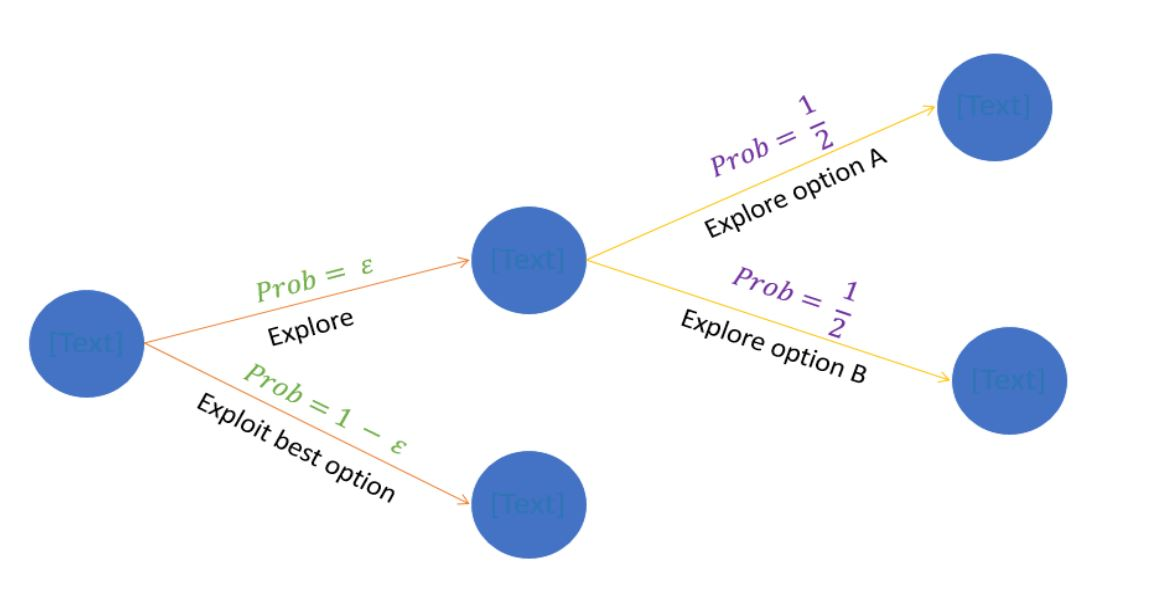
\includegraphics[width=1\linewidth]{epsilon greedy approach.jpg}
        \bfseries\caption{\textbf{\textcolor{blue}{Abordarea Epsilon-Greedy}}}\vspace{15mm}
         Imagine preluată din sursa: \textnormal{Analytics Vidhya. (2018, 24 septembrie). \emph{“Multi Armed Bandit Problem \& Its Implementation in Python.”} Consultat la adresa: \urlstyle{same} {\small \url{www.analyticsvidhya.com/blog/2018/09/reinforcement-multi-armed-bandit-scratch-python/}}}. 
\end{figure}
\newpage
\begin{center}
	    \textcolor{blue}{\section{\bfseries\scshape\textcolor{blue} {Funcționarea programului pentru experimentare}}}
\end{center}
Pentru a putea rula diverse simulări pentru aceaste abordări de rezolvare a soluției, am implementat un algoritm de generare aleatoare a datelor de intrare. Algoritmul pentru generarea datelor de intrare generează trei tipuri principale de valori cuprinse în plaja următoarelor intervale:
\begin{itemize}
\item\textbf{\textcolor{blue}{ num$\_$arms:}} 
\begin{itemize}
      \item Un număr întreg între 5 și 15. Acesta reprezintă numărul de "brațe"  în problemă. Cu cât este mai mare acest număr, cu atât este mai complexă problema.
\end{itemize}
\item\textbf{\textcolor{blue}{ num$\_$iterations:}} 
\begin{itemize}
      \item Un număr întreg între 1500 și 50000. Acesta reprezintă numărul total de iterații pe care algoritmul îl va efectua. Cu cât este mai mare acest număr, cu atât algoritmul are mai multe oportunități de a explora și de a învăța în timp. 
\end{itemize}
\item\textbf{\textcolor{blue}{ epsilon:}} 
\begin{itemize}
      \item Un număr real între 0.1 și 0.5. Controlează cât de mult se va explora în comparație cu exploatarea. Un epsilon mai mic încurajează exploatarea, în timp ce un epsilon mai mare încurajează explorarea.
\end{itemize}
\end{itemize}
Valorile varibilelor de mai sus sunt setate și pot fi modificate din fișierul $.py$. Datele de input sunt generate aleatoriu la fiecare iterație a buclei de generare a fișierelor de intrare, astfel existând varietate și diversitate în setul de date pe care metodele de rezolvare îl întâlnesc în timpul simulării. 
\begin{algorithm}
\caption{Random Input Generator}
\For{$i$ from $1$ to $num\_files$}{
    // Generate random values\\
    $num\_arms \leftarrow$ Random integer between 5 and 15\;\\
    $num\_iterations \leftarrow$ Random integer between 1500 and 50000\;\\
    $\varepsilon \leftarrow$ Round(Random float between 0.1 and 0.5, 2)\;\\
    // Create and write to the input file\\
    $file\_name \leftarrow$ Concatenate($output$\_$dir$, "$/input$" + $i$ + "$\cdot txt$")\;\\
    Open $file\_name$ with write mode\;\\
    Write $num\_arms$ to $file\_name$\;\\
    Write $num\_iterations$ to $file\_name$\;\\
    Write $\varepsilon$ to $file\_name$\;\\
    Close $file\_name$\;\\
}
\end{algorithm}
\newpage
	\begin{center}
	    \textcolor{blue}{\section{\bfseries\scshape\textcolor{blue}{Cazuri și date experimentale}}}
	\end{center}
Am ales să generez datele de intrare aleator, variind numărul de brațe, numărul total de iterații și parametrul epsilon. Acest lucru este o abordare bună pentru a testa rezistența algoritmilor în fața diverselor configurații ale problemei.\\\\
Numărul de iterații reprezintă de câte ori agenții fac alegeri și actualizează starea lor în cadrul simulării. În contextul mașinilor cu sloturi cu mai multe brațe (multi-arm bandit), fiecare iterație ar corespunde unei runde în care agenții decid ce braț să aleagă, trage brațul respectiv, obțin o recompensă și își actualizează estimările bazate pe acea experiență.\\
Cu cât numărul de iterații este mai mare, cu atât simularea rulează pe un număr mai mare de runde, permițând agenților să acumuleze mai multă experiență și să își ajusteze mai bine strategiile. Alegerea unui număr optim de iterații depinde de complexitatea problemei și de ritmul la care agenții pot învăța. Un număr prea mic de iterații ar putea să nu ofere suficient timp agenților pentru a descoperi strategiile optime, în timp ce un număr prea mare poate duce la timp de execuție crescut fără a aduce îmbunătățiri semnificative în performanță.\\\\
Am ales aceste intervale pentru a crea date de intrare variate și reprezentative pentru diferite scenarii ale problemei:
\begin{table}[ht]
\centering
\begin{tabular}{|c|c|c|c|}
\hline
\textbf{Număr Brațe} & \textbf{Număr Iterații} & \textbf{Epsilon} \\
\hline \{5, 15\} &\{1500, 50000\} &\{0.1,  0.5\} \\
\hline
\end{tabular}
 \bfseries\caption{\textbf{\textcolor{blue}{Intervalele de generare aleatoare a datelor de input}}}
\label{tab:input-data}
\end{table}
\begin{itemize}
\item\textbf{\textcolor{blue}{ Numărul de Brațe :}} 
\begin{itemize}
      \item Intervalul ales între 5 și 15 oferă o varietate suficientă de situații, de la cazuri simple cu doar cinci opțiuni până la situații mai complexe cu cincisprezece opțiuni. Astfel, putem evalua comportamentul agenților în fața unui număr diferit de alternative.
\end{itemize}
\end{itemize}
\begin{itemize}
\item\textbf{\textcolor{blue}{ Numărul de Iterații:}} 
\begin{itemize}
      \item Intervalul între 1500 și 50000 pentru numărul de iterații oferă o perspectivă asupra modului în care algoritmii evoluează în timp. Alegerea acestui interval permite simularea unor scenarii cu un număr rezonabil de iterații. Valorile mai mici pot fi asociate cu simulări mai scurte, în timp ce valorile mai mari pot simula experimente mai lungi. 
\end{itemize}
\end{itemize}
\begin{itemize}
\item\textbf{\textcolor{blue}{ Epsilon (pentru Epsilon-Greedy):}} 
\begin{itemize}
      \item Epsilon-ul este ales aleatoriu între 0.1 și 0.5. Prin variabilitatea acestui parametru, putem evalua cum comportamentul algoritmilor variază în funcție de gradul de explorare versus exploatare. Valori mai mici ale lui epsilon încurajează mai mult exploatarea, în timp ce valori mai mari încurajează explorarea.
\end{itemize}
\end{itemize}
Se creează un fișier de intrare pentru fiecare set de date generate. Numele fișierului este de forma input{\textit{i}}.txt, unde {\textit{i}} reprezintă numărul fișierului, iar numărul de fișiere generate este stabilit de utilizator, mai jos au fost generate 10 fișiere de input.\\ 
Pentru a menține informația vizibila, am configurat un fișier \textit{log.yml}, care este un fișier de configurare \textit{YAML} pentru setările de jurnalizare în Python, folosind modulul logging și generând un fișier de\textit{ output.log} cu informații despre generarea datelor.  
\begin{figure}[h]
    \centering
    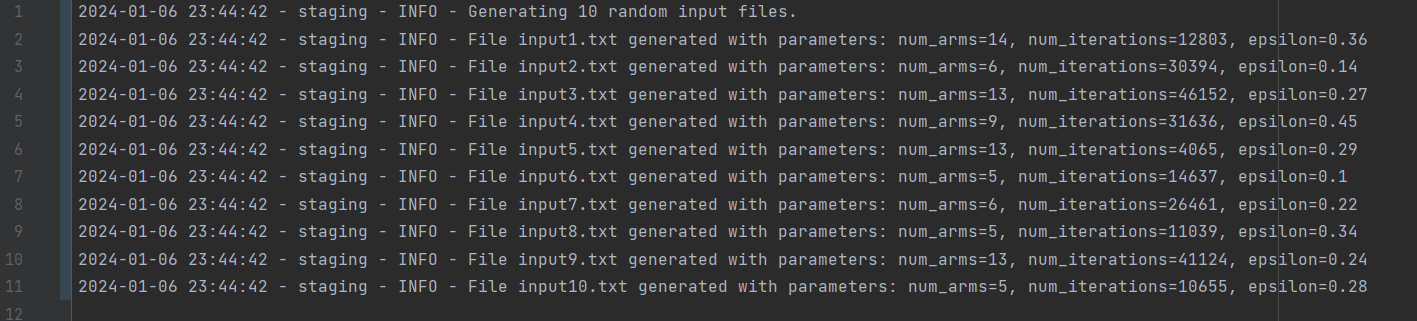
\includegraphics[width=1\linewidth]{input files generation.png}
    \textbf{  \caption{\textbf{\textcolor{blue}{Generarea aleatoare a fișierelor și datelor de intrare}}}}
\end{figure}
\begin{figure}[h]
    \centering
    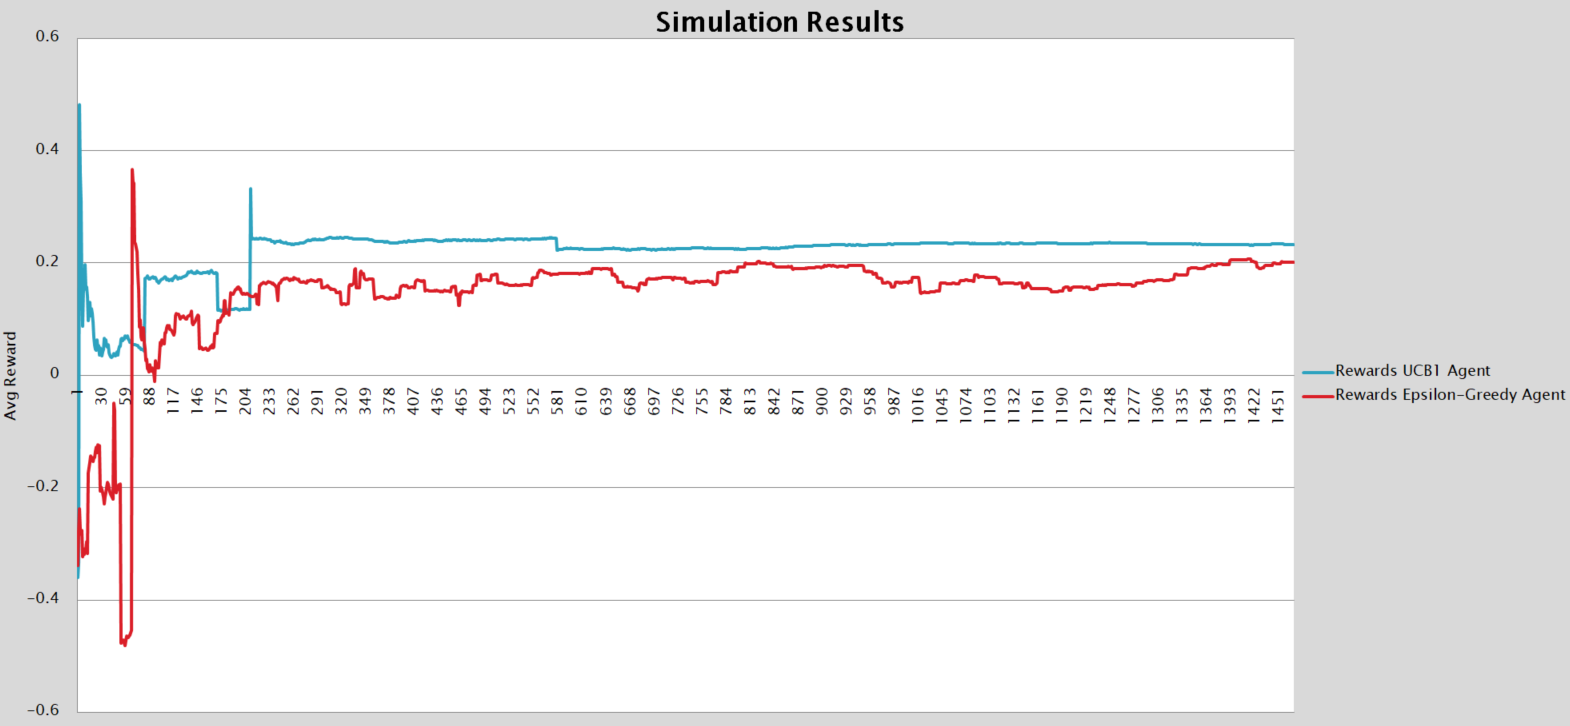
\includegraphics[width=1\linewidth]{simulation results.png}
    \bfseries\caption{\textbf{\textcolor{blue}{Compararea recompenselor medii ale agenților între iterații}}}
\end{figure}
\\Pentru fiecare iterație, se calculează recompensa medie a fiecărui agent. Acest lucru se face prin împărțirea sumei recompenselor obținute până la iterația respectivă la numărul total de trageri ale brațului (numărul total de iterații pentru acel braț).\\
Recompensa medie pentru ambii agenți începe să varieze semnificativ la început, ceea ce este tipic pentru etapa inițială de explorare în acest tip de simulări. În timp ce agenții continuă să exploreze și să învețe, varianța recompensei medii scade, iar valorile tind să se stabilizeze.\\
Pe măsură ce numărul de iterații crește, ambele linii par să se stabilizeze, indicând că agenții învață și se adaptează la mediu pentru a optimiza selecția brațelor pentru a maximiza recompensa.
Graficul sugerează că după o perioadă inițială de ajustare și explorare, performanța ambelor strategii se stabilizează, cu o recompensă medie care rămâne relativ constantă pe durata iterațiilor rămase. \\\\
În cazul acestui grafic, agentul UCB1 pare să aibă o performanță ușor mai bună pe termen lung, menținând o recompensă medie mai constantă și, în general, mai mare decât agentul Epsilon-Greedy.
Este important de menționat că, în timp ce ambele strategii se apropie de o recompensă medie stabilă, fluctuațiile inițiale sunt mai pronunțate pentru agentul Epsilon-Greedy, dar după această perioadă de ajustare inițială, recompensa se stabilizează la un nivel similar cu cel al agentului UCB1.\\ 
\begin{figure}[h]
    \centering
    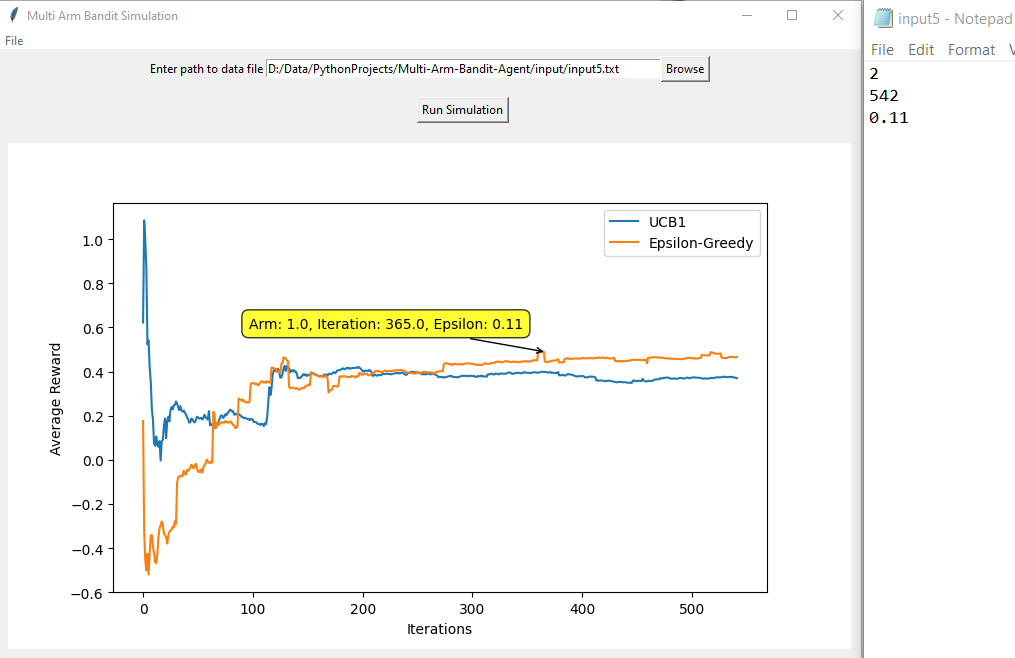
\includegraphics[width=1\linewidth]{plot generation.png}
    \bfseries\caption{\textcolor{blue}{\textbf{Simularea cu eps=0.11  rulând pe 542 iterații}}}
\end{figure}
\\La început, ambele algoritmi încep cu o recompensă negativă, ceea ce sugerează că au făcut selecții suboptimale de brațe. Pe măsură ce iterațiile progresează, ambele algoritmi îmbunătățesc performanța, cu recompensa medie crescând și stabilizându-se aproape de valoarea zero, cu oscilații mai mici. Aceasta indică faptul că algoritmii se adaptează și identifică brațele care oferă recompense mai bune.\\\\
\begin{figure}[h]
    \centering
    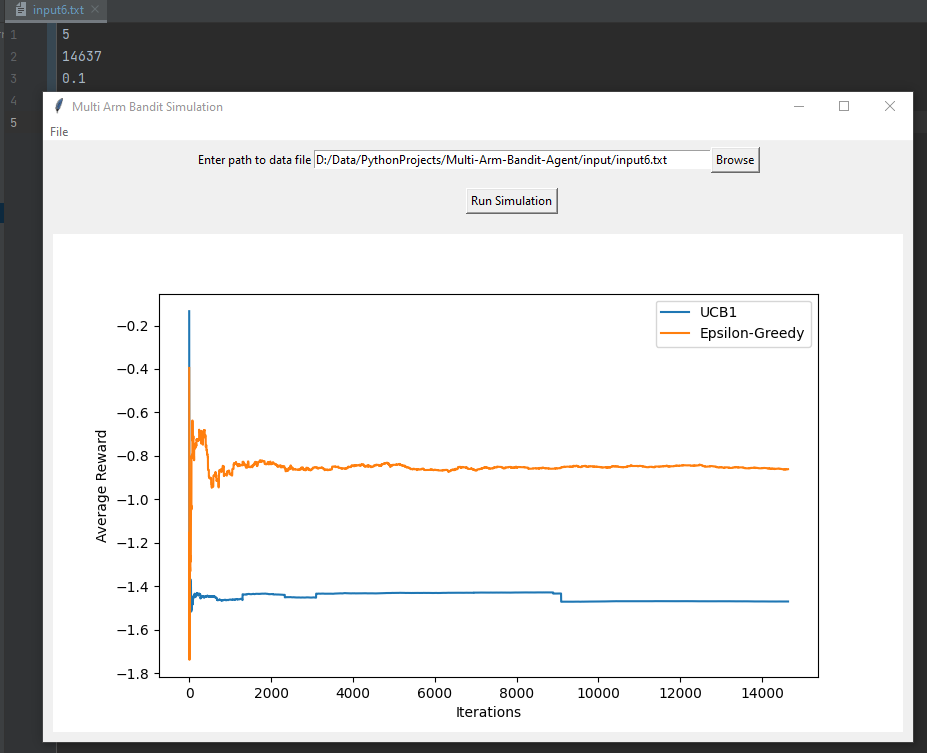
\includegraphics[width=1\linewidth]{plot generation 3.png}
    \bfseries\caption{\textcolor{blue}{\textbf{Simularea cu eps=0.1  rulând pe 14.637 iterații}}}
\end{figure}
\\Graficul arată „Recompensa Medie” pe verticală (axa Y) în raport cu „Iterațiile” pe orizontală (axa X). Valorile recompensei medii par să înceapă de la un nivel scăzut și să devină mai stabile pe măsură ce numărul de iterații crește. Linia albastră reprezintă strategia UCB1, iar linia portocalie reprezintă strategia Epsilon-Greedy. Pe măsură ce iterațiile progresează, ambele strategii par să converge către o recompensă medie constantă, cu strategia Epsilon-Greedy având o recompensă puțin mai mică decât UCB1, sugerând că UCB1 poate fi strategia mai performantă în acest scenariu particular. Media este în general negativă  și se stabilizează relativ repede după o scădere inițială.\\
\newpage
\begin{figure}[h]
    \centering
    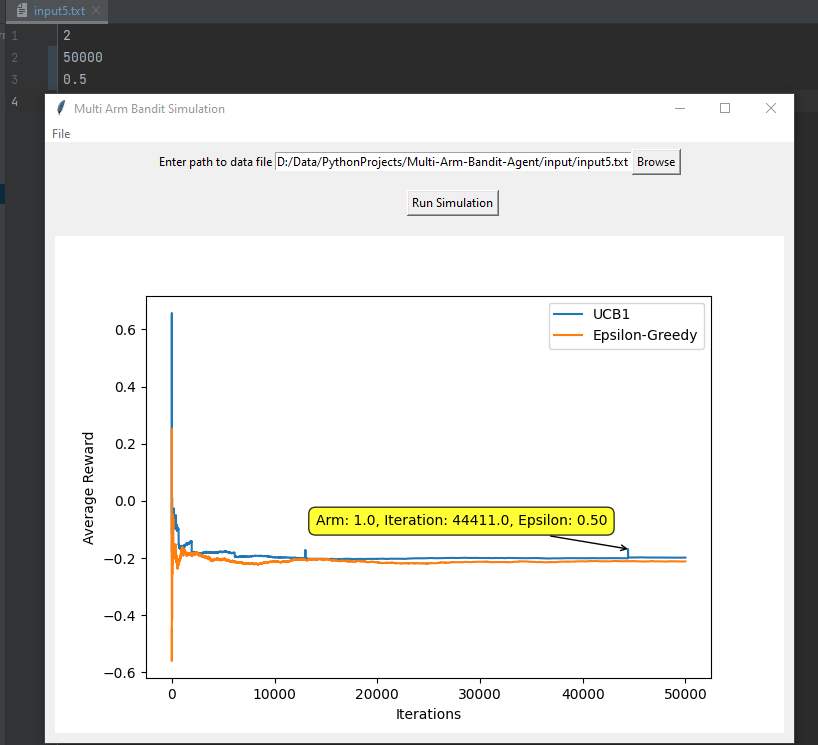
\includegraphics[width=1\linewidth]{plot generation 2.png}
    \bfseries\caption{\textcolor{blue}{\textbf{Simularea cu eps=0.5 rulând pe 50.000 iterații}}}
\end{figure}
Graficul indică faptul că ambele strategii au avut o perioadă de învățare inițială (indicată de o scădere abruptă), după care recompensele lor medii s-au stabilizat. Linia albastră (UCB1) și linia portocalie (Epsilon-Greedy) sunt foarte apropiate una de alta pe parcursul simulației, sugerând că performanța celor două strategii este similară în acest scenariu.
Un detaliu adițional este afișat în colțul din dreapta jos al graficului, care indică un "braț" (probabil cel mai bun braț determinat de simulare), numărul iterației (44.411), și valoarea epsilon (0.50), care este un parametru pentru strategia Epsilon-Greedy ce determină cât de des algoritmul va explora acțiuni noi în loc să exploateze cea mai bună acțiune cunoscută până în momentul respectiv.
\newpage
\begin{figure}[h]
    \centering
    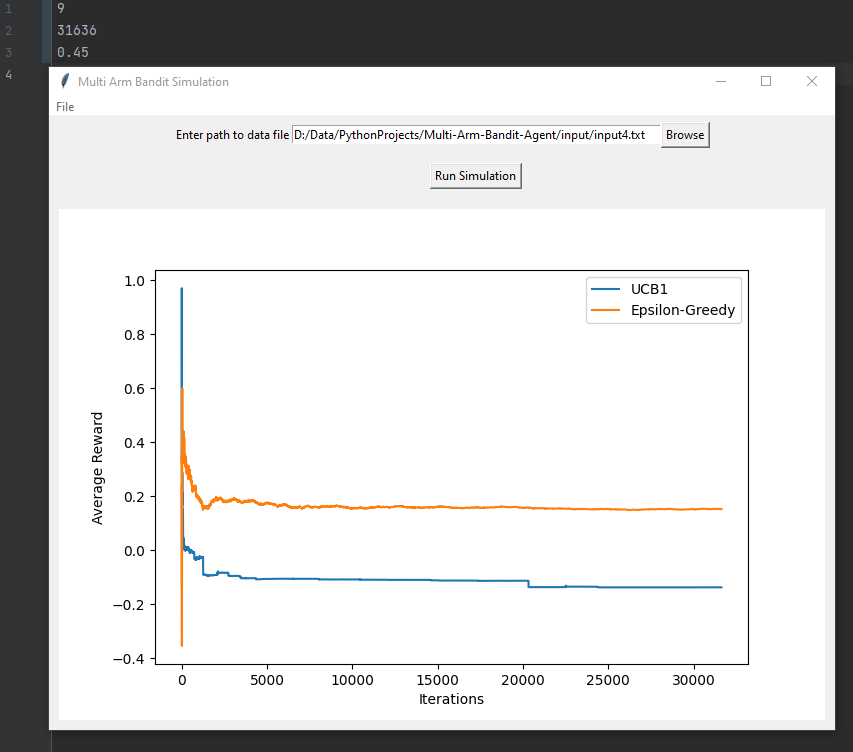
\includegraphics[width=1\linewidth]{plot generation 4.png}
    \bfseries\caption{\textcolor{blue}{\textbf{Simularea cu eps=0.45 rulând pe 31.636 iterații}}}
\end{figure}
La începutul graficului, există o scădere accentuată pentru ambele strategii, ceea ce indică o perioadă inițială de explorare sau învățare, unde algoritmii experimentează pentru a găsi acțiuni cu recompense mai bune. După această scădere inițială, ambele linii se aplatizează și devin relativ stabile, ceea ce sugerează că ambele strategii au ajuns la o anumită performanță constantă după un număr inițial de iterații.\\
UCB1 și Epsilon-Greedy par să aibă performanțe similare până la aproximativ 5.000 de iterații, după care UCB1 menține o recompensă medie ușor mai constantă comparativ cu Epsilon-Greedy. Aceasta poate sugera că UCB1 gestionează mai bine echilibrul dintre exploatare și explorare în acest scenariu de simulare.\\\\\\
\begin{figure}[h]
    \centering
    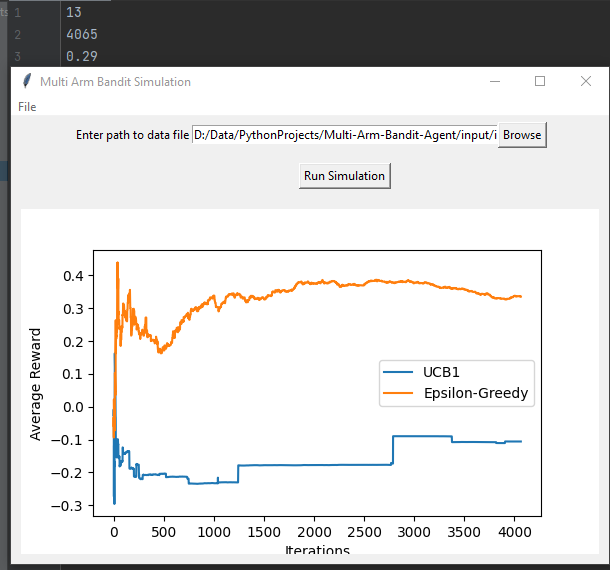
\includegraphics[width=0.95\linewidth]{plot generation 5.png}
    \bfseries\caption{\textcolor{blue}{\textbf{Simularea cu eps=0.29 rulând pe 4.065 iterații}}}
\end{figure}
\\În faza inițială, ambele strategii încep cu o variație mare a recompensei medii, cu Epsilon-Greedy având o scădere inițială, apoi o creștere rapidă, iar UCB1 începe cu o scădere și apoi se stabilizează. \\\\
Această volatilitate inițială este tipică în fazele de explorare inițiale ale algoritmilor de învățare, unde algoritmul testează diferite brațe pentru a estima valoarea lor.
Pe măsură ce numărul de iterații crește, linia portocalie indică faptul că recompensa medie pentru strategia Epsilon-Greedy crește și se stabilizează la o valoare pozitivă. 
Aceasta sugerează că strategia Epsilon-Greedy a început să identifice și să exploateze brațele cu recompense mai mari.\\\\
Linia albastră pentru UCB1 se stabilizează la o recompensă medie mai scăzută decât Epsilon-Greedy și rămâne relativ constantă pe parcursul simulării. Acest lucru ar putea indica faptul că, în această simulare și cu parametrii dați, UCB1 nu a performant la fel de bine ca Epsilon-Greedy. Rezultatele arată că, pentru această simulare specifică și setul de parametri, strategia Epsilon-Greedy a reușit să obțină o recompensă medie mai mare decât UCB1, indicând posibil o adaptare mai bună la acest mediu de simulare sau o mai bună exploatare a informațiilor obținute în timpul fazei de explorare.\\\\
\begin{table}[ht]
    \centering
    \begin{tabular}{|c|c|c|c|}
    \hline \textbf{Iterația} & \textbf{Timp execuție} & \textbf{Număr brațe}  & \textbf{Valoarea epsilon} \\
    \hline  4.065     &  2.24 \textit{sec}    & 13   &  $\varepsilon = $ 0.29\\
    \hline  10.655    &  5.73  \textit{sec}   &  5   &  $\varepsilon = $ 0.28\\
    \hline  11.039    &  5.52 \textit{sec}    &  5   &  $\varepsilon = $ 0.34\\
    \hline  12.803    &  7.04 \textit{sec}    &  14  &  $\varepsilon = $ 0.36\\
    \hline  14.637    &  8.28 \textit{sec}    &  5   &  $\varepsilon = $ 0.1\\
    \hline  26.461    &  14.42 \textit{sec}   &  6   & $\varepsilon = $ 0.22\\
    \hline  30.394    &  16.48 \textit{sec}   &  6   &  $\varepsilon = $ 0.14\\
    \hline  31.636    &  15.78 \textit{sec}   &  9   & $\varepsilon = $ 0.45\\
    \hline  41.124    &  22.97 \textit{sec}   &  13  &  $\varepsilon = $ 0.24\\
    \hline  46.152    &  25.55 \textit{sec}   &  13  &  $\varepsilon = $ 0.27\\
    \hline
    \end{tabular}
    \bfseries\caption{\textbf{\textcolor{blue}{Timpul de execuție pe iterații}}}
    \label{tab:execution-time}
\end{table}
\\\\Se poate observa că timpul de execuție crește  pe măsură ce numărul de iterații crește. Acest lucru era de așteptat, deoarece fiecare iterație implică un număr de runde mai mare în simulare, iar acest proces se repetă de fiecare dată.\\
În general, o creștere a timpului de execuție odată cu creșterea numărului de iterații poate sugera că simularea devine mai intensivă pe măsură ce agentul acumulează mai multă experiență și ajustează strategiile sale.\\\\
Este important de remarcat că valoarea epsilon și numărul de brațe par, de asemenea, să influențeze timpul de execuție. Itreații cu un număr mai mare de brațe au tendința de a avea timpuri de execuție mai mari, iar valori mari ale lui epsilon par să fie asociate cu timpuri de execuție mai lungi în unele cazuri. Aceste observații sugerează că complexitatea problemei poate crește odată cu variabilele precum numărul de brațe și valoarea epsilon, având un impact asupra timpului necesar pentru a realiza iterațiile.
\newpage
\begin{center}
	\textcolor{blue}{\section{\bfseries\scshape\textcolor{blue}{Probleme întâmpinate}}}
\end{center}
Înainte de a aborda și soluționa problema, a fost nevoie sa investesc ceva timp pentru a face o cercetare amănunțită și detaliată, care să mă ajute să mă pot decide asupra limbajului de programare și a editorului folosit.\\\\
Unele din noțiunile importante descoperite de mine cercetând, care m-au ajutat în rezolvarea acestei teme, sunt urmatoarele:

\begin{itemize}
\item\textbf{\textcolor{blue}{Explorare vs. Exploatare: }} 
\begin{itemize}
      \item  Este un concept fundamental în problemele de sloturi cu mâini multiple (multi armed bandit). Alegerea între a explora opțiuni noi și a exploata cele existente este crucială pentru obținerea unor rezultate optime.
\end{itemize}
\end{itemize}
\begin{itemize}
\item\textbf{\textcolor{blue}{Algoritmul Epsilon-Greedy:}} 
\begin{itemize}
      \item  Un algoritm simplu și eficient care se bazează pe ideea de a alege cu probabilitatea epsilon să explorezi și cu probabilitatea 1-epsilon să exploatezi. Este o opțiune importantă în abordarea mea.
\end{itemize}
\end{itemize}
\begin{itemize}
\item\textbf{\textcolor{blue}{Algoritmul UCB (Upper Confidence Bound):}} 
\begin{itemize}
      \item  Este un alt algoritm popular, care se concentrează pe exploatare, alegând acțiunile care au cea mai mare "încredere" (o combinație de recompensă medie și incertitudine).
\end{itemize}
\end{itemize}
\begin{itemize}
\item\textbf{\textcolor{blue}{Analiza și Vizualizarea Rezultatelor: }} 
\begin{itemize}
      \item  Înțelegerea rezultatelor și modul în care algoritmii iau decizii.
\end{itemize}
\end{itemize}
Instalarea mediului de dezvoltare PyCharm nu a fost dificilă, totul fiind open source și doar executând un fișier .exe. Am găsit un ghid folositor pe site-ul companiei JetBrains care oferea informații pentru toți pașii necesari de urmat, cum ar fi: instalarea de Python, în cazul meu versiunea 3.10, de asemenea distribuția Anaconda a fost ușor de instalat, descărcat sub formă de arhivă și pornit, având informații atât pentru windows, cât și pentru alte sisteme de operare.\\ 
Ghidul a oferit și configurările care trebuiesc realizate pentru ca totul să funcționeze complet.\\\\
Cea mai mare dificultate pe care am avut-o a fost să stabilesc modul de soluționare al problemei, astfel încât să fie cât mai eficient.

\begin{center}
	\textcolor{blue}{\section{\bfseries\scshape\textcolor{blue}{ Proiectarea și implementarea}}}
\end{center}
\textcolor{purple}{\subsection{\itshape \textcolor{purple}{Implementare}}}
\textbf{Principalele funcționalități implementate sunt următoarele:}
\begin{itemize}
\item\textbf{\textcolor{blue}{Interfața Grafică (GUI): }} \vspace{2mm}
\begin{itemize}
      \item  Am creat o interfață grafică folosind biblioteca Tkinter pentru a oferi utilizatorului o modalitate intuitivă de a interacționa cu simularea agentului cu mai multe brațe.\vspace{2mm}
      \item  Elementele GUI includ un câmp pentru a introduce calea către fișierul de date, un buton pentru a rula simularea și o fereastră pentru afișarea plot-urilor rezultate.\vspace{2mm}
      \item  Interfața grafică permite monitorizarea în timp real a parametrilor și rezultatelor simulărilor, facilitând procesul de depanare și îmbunătățire continuă.\vspace{2mm}
\end{itemize}

\item\textbf{\textcolor{blue}{Citirea Datelor de Intrare: }} \vspace{2mm}
\begin{itemize}
      \item  Am implementat o funcționalitate pentru a permite utilizatorului să încarce un fișier de date care conține informații despre simulare, cum ar fi numărul de brațe, numărul total de iterații și epsilon (în cazul algoritmului Epsilon-Greedy).\vspace{2mm}
\end{itemize}

\item\textbf{\textcolor{blue}{Simularea Agentului cu Mai Multe Brațe:}} \vspace{2mm}
\begin{itemize}
      \item Am creat o clasă MultiArmedBandit pentru a reprezenta agentul cu mai multe brațe. Aceasta stochează informații despre fiecare braț și oferă funcționalitate pentru a trage de aceste brațe și a obține recompense.\vspace{2mm}
\end{itemize}

\item\textbf{\textcolor{blue}{Implementarea Agenților:}} \vspace{2mm}
\begin{itemize}
      \item \textbf{\textcolor{red}{UCB1 Agent:}} \vspace{2mm}
      \begin{itemize}
         \item  Am implementat algoritmul UCB1 care alege brațul cu valoarea estimată maximizată, luând în considerare și explorarea. Am actualizat valoarea estimată a fiecărui braț în funcție de recompensele obținute.\vspace{2mm}
      \end{itemize}
    \item \textbf{\textcolor{red}{Epsilon-Greedy Agent:}} \vspace{2mm}
      \begin{itemize}
         \item  Am implementat algoritmul Epsilon-Greedy, care are două moduri de acțiune: exploatare (alege brațul cu valoarea estimată maximă) și explorare (alege un braț aleator dacă epsilon este respectat). A fost actualizată valoarea estimată pentru brațul ales.\vspace{4mm}
      \end{itemize}
\end{itemize}

\item\textbf{\textcolor{blue}{Implementarea Generatorului de Date: }} \vspace{2mm}
\begin{itemize}
      \item  Am implementat o funcționalitate pentru a permite utilizatorului să genereze fișiere de intrare, cât și date de intrare aleatorii pentru simulările cu cei doi algoritmi de mai sus. Datele de intrare sunt cuprinse în anumite intervale specifice, valorile acestor intervale pot fi modificate de câtre utilizator.\vspace{2mm}
\end{itemize}

\item\textbf{\textcolor{blue}{Simularea și Colectarea Datelor:}} \vspace{2mm}
\begin{itemize}
      \item Am simulat mai multe iterații în care agenții au ales brațe și au obținut recompense de la bandit. Am colectat date precum recompensele medii pentru fiecare agent în fiecare iterație.\vspace{2mm}
\end{itemize}

\item\textbf{\textcolor{blue}{Generarea și Afișarea Plot-urilor:}} \vspace{2mm}
\begin{itemize}
      \item Am utilizat biblioteca Matplotlib pentru a genera plot-uri care compară performanța agenților UCB1 și Epsilon-Greedy în timpul simulării.\vspace{2mm}
       \item Am afișat aceste plot-uri în interfața grafică pentru ca utilizatorul să poată vedea și înțelege rezultatele simulării.\vspace{2mm}
        \item Graficele și ploturile pot fi prezentate în mod mai estetic și ușor de înțeles, facilitând interpretarea rezultatelor.\vspace{2mm}
\end{itemize}

\item\textbf{\textcolor{blue}{ Salvarea Plot-urilor:}} \vspace{2mm}
\begin{itemize}
      \item Am adăugat opțiunea pentru utilizator de a salva plot-urile generate într-un director de ieșire specific.\vspace{2mm}
\end{itemize}
\end{itemize}
Din fericire pentru mine, faptul că am ceva experientă, atât cu limbajul de programare, cât și cu mediul de dezvoltare și distribuția folosită a fost de mare ajutor, întrucât nu a fost necesară portarea dintr-un limbaj de progamare în alt limbaj de programare, și s-au putut implementa toate funcționalitățile utilizând același limbaj de programare, Python.\\\\
\textbf{\textit{Aplicația este dezvoltată de la zero, iar pentru acele două abordări, Epsilon-Greedy și UCB 1 o principală resursă de inspirație poate fi aceesată la următorul link:\\}}
“Bandit\_simulations/Python/Multiarmed\_bandits at Master · Kfoofw/Bandit\_simulations.” GitHub, \urlstyle{same} {\small \url{https://github.com/kfoofw/bandit_simulations/tree/master/python/multiarmed_bandits}}. Accessed 6 Jan. 2024.
\vspace{20mm}

\textcolor{purple}{\subsection{\itshape \textcolor{purple}{Proiectare}}}
\begin{figure}[h]
    \centering
    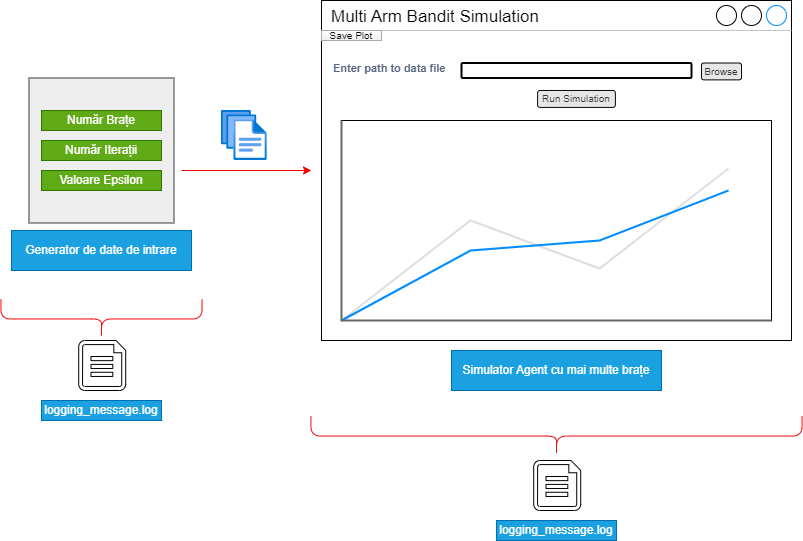
\includegraphics[width=1\linewidth]{toolchain workflow.drawio.png}
    \bfseries\caption{\textcolor{blue}{\textbf{Modul de lucru al toolchain-ului implementat}}}
\end{figure}
Imaginea încărcată reprezintă o diagramă de flux a procesului pentru o simulare a agenților cu brațe multiple. Diagrama descrie cum intrările generate de un generator de date sunt folosite de simulatorul problemei și cum rezultatele sunt apoi înregistrate și afișate.\\
\begin{enumerate}
    \item \textcolor{blue}{\textbf{Generatorul de date de intrare}}
    \begin{itemize}
        \item Utilizatorul rulează aplicația generatorului de date, care este un script dezvoltat în Python.
        \item Parametrii, cum ar fi intervalele pentru date, sunt hardcodate direct în codul generatorului.
        \item Generatorul rulează, generează datele conform intervalelor specificate și salvează aceste date în fișiere, unde numărul maxim de generare al fișierelor este hadcodat în cod.\\\\
    \end{itemize}
    \item \textcolor{blue}{\textbf{Simulatorul Agentului cu Interfață Grafică}}
    \begin{itemize}
        \item Utilizatorul deschide aplicația simulatorului cu interfață grafică.
        \item Interfața grafică permite utilizatorului să încarce fișierul de date generat anterior.
        \item După configurare, utilizatorul poate rula simularea, iar interfața grafică va afișa în timp real rezultatele sub formă de grafic.
        \item Salvarea graficului este disponibilă pentru păstrarea rezultatelor.\\
    \end{itemize}
    \item \textcolor{blue}{\textbf{Interacțiune între Aplicații}}
    \begin{itemize}
        \item Generatorul de date rulează independent și poate fi rulat ori de câte ori este nevoie pentru a genera noi seturi de date.Acesta este blocul de unde începe procesul. Se pare că generatorul creează date de intrare aleatorii care vor fi folosite în simulare. Valorile specifice sunt pentru "Număr Brațe", "Număr Iterații" și "Valoare Epsilon".Valorile generate sunt scrise într-un fișier de intrare, așa cum indică iconița cu un document și o săgeată care indică spre dreapta.
        \item Utilizatorul încarcă datele generate în simulator, iar interfața grafică a simulatorului permite experimentarea cu aceste date și observarea impactului asupra agenților.Aici este prezentată interfața grafică a utilizatorului (GUI) pentru simulator. Se poate vedea o zonă unde utilizatorul poate introduce calea către fișierul de date și un buton pentru a rula simularea. Există și o zonă de plotare grafică unde rezultatele simulării sunt afișate sub formă de grafic.
        \item Prin această abordare, generatorul de date funcționează într-un mod automatizat, iar datele generate sunt apoi utilizate în mod flexibil în simulatorul cu interfață grafică pentru analize și simulări interactive.Rezultatele sunt afișate grafic.Rezultatele simulării sunt, de asemenea, înregistrate într-un fișier de log, așa cum indică săgeata roșie și iconița documentului de jos. Acest fișier de log conține detalii suplimentare despre execuția simulării, cum ar fi erorile, avertismentele și alte mesaje informative.
    \end{itemize}
\end{enumerate}
\textcolor{purple}{\subsection{\itshape \textcolor{purple}{Viitoare îmbunătățiri}}}
\begin{enumerate}
    \item Pentru generatorul de date, pe viitor ar fi util să aibă posibilitatea să configureze intervalele pentru date direct dintr-un fișier de configurare (json/xml/txt, etc) și dat ca parametru prin command line interface.
    \item Pentru simulatorul agentului, adăugarea unor opțiuni suplimentare pentru vizualizarea datelor, cum ar fi histograma recompenselor sau evoluția estimărilor brațelor în timp.
    \item Extinderea simulatorului pentru a accepta și simula datele folosind mai multe metode, oferind utilizatorilor opțiuni variate pentru testare.
    \item Optimizarea algoritmiilor, pentru a asigura o performanță mai bună, în special în cazul unor seturi de date mai mari.
\end{enumerate}
\begin{center}
	\textcolor{blue}{\section{\bfseries\scshape\textcolor{blue}{ Concluzii}}}
\end{center}
 Această temă a constituit cu adevărat o provocare stimulantă, în care am depus eforturi constante pentru a absorbi cât mai multe detalii și noțiuni esențiale. De la înțelegerea cerințelor, la abordarea meticuloasă a problemei și implementarea soluției, fiecare etapă a fost o oportunitate de a învăța și de a evolua. Am investit timp în a dezvolta nu doar o soluție funcțională, ci și o înțelegere profundă a contextului și a implicațiilor fiecărui pas pe care l-am făcut. Astfel, consider că această experiență nu doar că mi-a consolidat cunoștințele, dar m-a și ajutat să experimentez mai mult acest domeniu.\\\\
 În urma acestei teme, mi-am îmbunătățit abilitățile de codare în limbajul Python,ci și o extindere a noțiunilor de sintaxă în LaTeX, prin utilizarea platformei online Overleaf. A fost o oportunitate de a explora și de a mă adapta la diferite aspecte ale programării și documentării, contribuind astfel mai mult la dezvoltarea mea în acest domeniu.\\\\
Acest proiect nu doar că mi-a consolidat competențele în Python, ci m-a și deschis către o lume fascinantă a sistemelor multi-agent, machine learning și metodelor de învățare prin recompensare. Prin el, am dobândit nu doar cunoștințe tehnice, ci și o înțelegere mai profundă a modului în care aceste concepte pot fi aplicate în practică.Am optat pentru dezvoltarea în limbajul Python datorită naturii sale concise și a facilității de înțelegere a implementărilor.\\
Alegerea acestui limbaj a fost determinată de dorința de a îmbunătăți în mod semnificativ abilitățile mele specifice în Python. Prin folosirea acestui limbaj, am avut oportunitatea de a explora și de a mă aprofunda în caracteristicile sale tehnice, precum manipularea eficientă a structurilor de date, gestionarea fluxurilor de control și utilizarea extensivă a bibliotecilor specializate. În acest fel, am fost capabil să aduc o anumită eleganță și eficiență în implementarea mea, cu un accent deosebit pe claritatea codului și pe maximizarea potențialului oferit de limbajul Python.\\\\
O altă concluzie este reprezentată de termenul limită al temei de casă. Acest parametru a avut un impact mai bun asupra organizării timpului, cât și asupra unei coordonari mai responsabile a celorlalte aspecte realizate pentru a rezolva această temă, ceea ce constituie un beneficiu mai amplu pentru dezvoltarea mea în acest domeniu.\\\\
Deși am avut câteva bătăi de cap în elaborarea soluției, m-am bucurat să găsesc o varietate de articole și resurse online care mi-au luminat calea. Evident, au existat și mici piedici în stadiul inițial al implementării, dar am reușit să le rezolv și să obțin o soluție funcțională pentru sarcina propusă.
Am încercat să respect fiecare cerință din metodologie, astfel încât să pot descrie fiecare parametru corespunzator acesteia în funcție de implementările, abordarea și rezultatele pe care le-am justificat mai sus. Am considerat crucial să aprofundez fiecare aspect al cerințelor, evidențiind nu doar rezultatele finale, ci și procesul detaliat care a condus la acestea.\\
Sunt mulțumită de rezultatele obținute în cadrul acestui proiect, care m-au îmbogățit nu doar cu abilități esențiale în Python, la care cu siguranță voi apela și în viitor, ci și cu o perspectivă complet nouă asupra sistemelor multi-agent, machine learning și metodelor de învățare prin recompensare.
\begin{center}
	\textcolor{blue}{\section{\bfseries\scshape\textcolor{blue}{ Bibliografie }}}
\end{center}
 Mai jos se pot observa câteva referințe bibliografice, documente, site-uri web, referințe ce au ajutat în parcurgerea, documentarea și înțelegerea mai amplă a temei de casă.
\begin{thebibliography}{8}
  \bibitem{slivkins-intro-mab}
     Slivkins, Aleksandrs. “Introduction to Multi-Armed Bandits.” Foundations and Trends® in Machine Learning, vol. 12, no. 1-2, 2019, pp. 1–286,  \urlstyle{same} {\small \url{https://doi.org/10.1561/2200000068}}. 
     
  \bibitem{slivkins-intro-mab}
    “Bandit\_simulations/Python/Multiarmed\_bandits at Master · Kfoofw/Bandit\_simulations.” GitHub, \urlstyle{same} {\small \url{https://github.com/kfoofw/bandit_simulations/tree/master/python/multiarmed_bandits}}. Accessed 6 Jan. 2024.
    
  \bibitem{wong2020solving}
    Wong, Anson. “Solving the Multi-Armed Bandit Problem.” Medium, 10 Feb. 2020, 
    \urlstyle{same} {\small \url{https://towardsdatascience.com/solving-the-multi-armed-bandit-problem-b72de40db97c}}.
    
  \bibitem{m2023solving}
    M, Vikram. “Solving Multi-Arm Bandits with Python.” Analytics Vidhya, 28 Feb. 2023, 
    \urlstyle{same} {\small \url{www.analyticsvidhya.com/blog/2023/02/solving-multi-arm-bandits-with-python/}}.
    
  \bibitem{javatpoint-rl-tutorial}
     Reinforcement Learning Tutorial - Javatpoint. \urlstyle{same} {\small \url{www.javatpoint.com/reinforcement-learning}}. 
 
  \bibitem{domino-rl-k-armed}
    Reinforcement Learning: The K-Armed Bandit Problem. Domino.ai,\urlstyle{same} {\small \url{domino.ai/blog/k-armed-bandit-problem}}. Accessed 30 Dec. 2023.

  \bibitem{multi-armed-bandit-wikipedia}
     Multi-Armed Bandit. Wikipedia, 27 Dec. 2023, \urlstyle{same} {\small  \url{en.wikipedia.org/wiki/Multi-armed_bandit#:~:text=In%20probability%20theory%20and%20machine}}.
   
  \bibitem{mahajan-teneketzis}
    Mahajan, Aditya, and Demosthenis Teneketzis. Multi-Armed Bandit Problems.
    \urlstyle{same} {\small  \url{https://web.eecs.umich.edu/~teneket/pubs/MAB-Survey.pdf}}. 
    
  \bibitem{overleaf-tutorials}
     Overleaf Tutorials.  \urlstyle{same} {\small  \url{www.overleaf.com/learn/latex/Tutorials}}. 

  \bibitem{oeis-math-symbols}
    List of LaTeX Mathematical Symbols - OeisWiki. \urlstyle{same} {\small \url{oeis.org/wiki/List_of_LaTeX_mathematical_symbols}}. 
    
  \bibitem{anaconda-pycharm-doc}
    Using PyCharm — Anaconda Documentation.\urlstyle{same} {\small \url{docs.anaconda.com/free/anaconda/ide-tutorials/pycharm/}}. Accessed 30 Dec. 2023.

  \bibitem{python-docs}
    Python Documentation Contents — Python 3.8.3 Documentation.\urlstyle{same} {\small \url{docs.python.org/3/contents.html}}.
    
  \bibitem{teeriaho-sofia}
    Teeriaho, Sofia. “Sofiateeriaho/MultiArmedBandit.” GitHub, 17 Feb. 2022, \urlstyle{same} {\small \url{github.com/sofiateeriaho/MultiArmedBandit}}. Accessed 30 Dec. 2023. 

  \bibitem{tk-python}
   “Tkinter - the Python Interface for Tk | Tkinter | Python-Course.eu.” Python-Course.eu, \urlstyle{same} {\small \url{python-course.eu/tkinter/}}. Accessed 1 Ian. 2024. 
\end{thebibliography}

\textbf{\large \textcolor{black}{\bfseries{$\blacktriangleleft$}  Ianuarie 2024. $\blacktriangleright$}}

\end{document}